% Dekatron
% Author Rohin T Narayan. 
% http://rohin.tn.googlepages.com. rohin.tn a t gmail.com.%
%%%%%%%%%%%%%%%%%%%%%%%%%%%%%%%%%%%%%%%%%%%%%%%%%%%%%%%%%%%%%%%%%%%%%%%%%%%%%%
%%%%%%%%%%%%%%%%%%%%%%%%%%%%%%%%%%%%%%%%%%%%%%%%%%%%%%%%%%%%%%%%%%%%%%%%%%%%%%
%This work is copyrighted under creative commons attribute license.
%You are free to copy, use, transmit this work either modified or original
%provided you leave the above header in the source code.

\documentclass{article}
\usepackage{xcolor}
\usepackage{tikz}
\usetikzlibrary{scopes}
\usepackage{verbatim}

\begin{comment}
:Title: Dekatron

Dekatrons were used by Experimental Nuclear and High Energy physicists long before
they embraced supreme technology of Digital signal processing and
computers. This is the scheme of electrodes in a dekatron tube which was
originally done for the lab manual at my University.
\end{comment}

\begin{document}
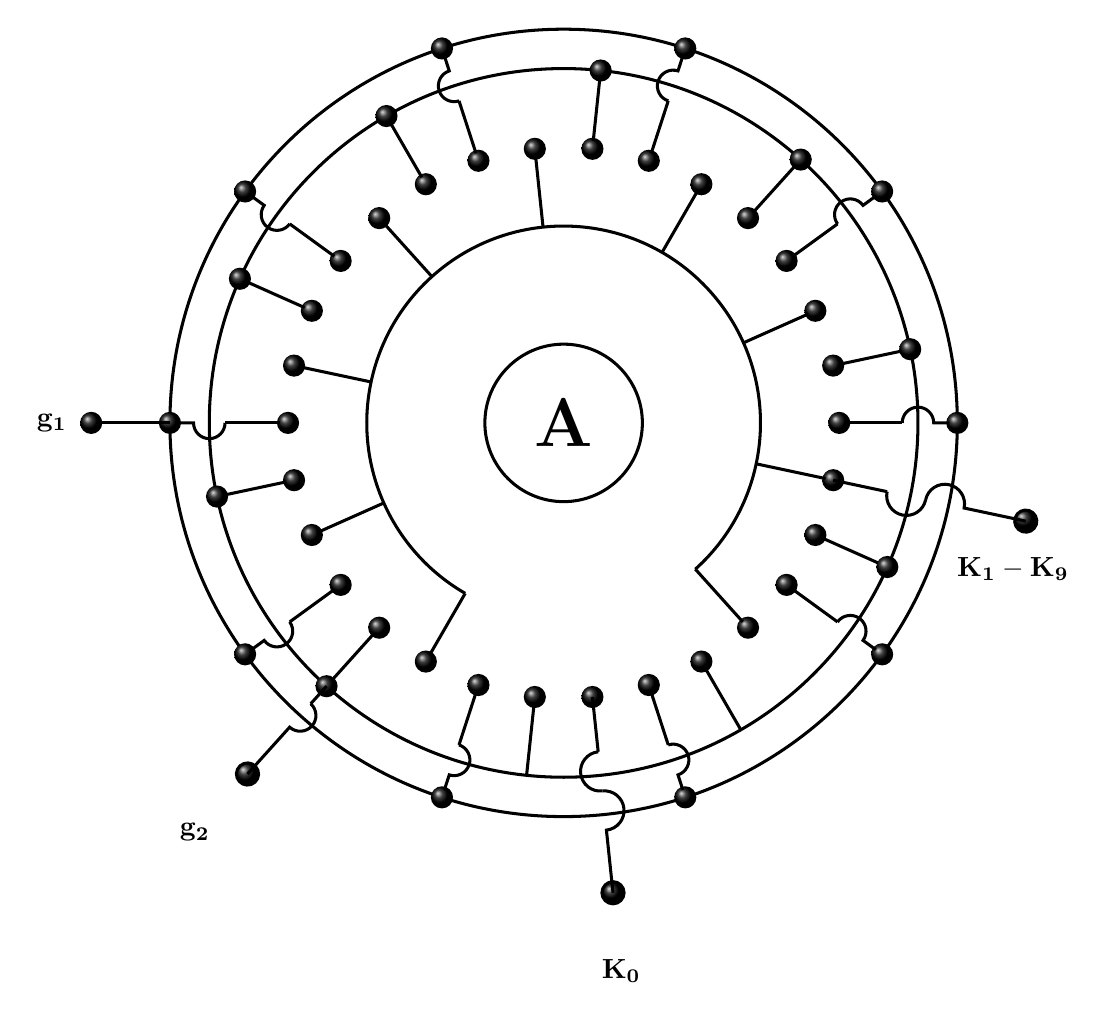
\begin{tikzpicture}[line width=1.1pt]
    \draw(0,0) circle(5cm);
    \draw(0,0) circle(1cm);
    \draw(0,0) node {\Huge$\mathbf{A}$};
    \draw(0,0) circle(4.5cm);
    \draw(-48:2.5) arc(-48:240:2.5cm);
    %% The outer nodes
    \foreach \x in {36,72,...,360}
    	\shade[ball color=black](\x:5) circle(4pt);
    \foreach \nodes in {12,24,...,360}
    	\shade[ball color=black](\nodes:3.5) circle(4pt);
    %%% The connecting nodes
    \foreach \angle in {-48,-12,...,240}
    	\draw(\angle:2.5) --++(\angle:0.9cm);
    %%% outer interconnects
    \foreach \angle in {-24,12,...,306}
    	\draw(\angle:3.6) --++(\angle:0.9cm);
    \foreach \y in {-24,12,...,240}
    	\shade[ball color=black](\y:4.5cm) circle(4pt);

    %% outer most connections
    \foreach \angle in{-36,0,...,306}
    	\draw(\angle:4.9cm) --(\angle:4.7cm) [rotate=\angle]arc(0:180:0.20cm);
    \foreach \angle in{-36,0,...,306}
    	\draw(\angle:4.3cm) --(\angle:3.6cm);
    %% Outer connects and leads
    \shade[ball color=black](276:6) circle(4pt);
    \draw(276:6)circle(4pt)--(276:5.2)[rotate=276]arc(0:180:0.25cm);
    \draw(276:7)node {$\mathbf{K_0}$};
    \draw(276:4.2)[rotate=276]arc(180:360:0.25cm);
    \draw(276:4.2)--(276:3.5);

    %% Exploitation of circular symmetry of the required figure

    {[rotate=72]
    	\shade[ball color=black](276:6) circle(4pt);
    	\draw(276:6)circle(4pt)--(276:5.2)[rotate=276]arc(0:180:0.25cm);
    	\draw(270:6)node {$\mathbf{K_1-K_9}$};
    	\draw(276:4.2)[rotate=276]arc(180:360:0.25cm);%%%
    	\draw(276:4.2)--(276:3.5);
    }

    {[rotate=-48]
    	\shade[ball color=black](276:6) circle(4pt);
    	\draw(276:6)circle(4pt)--(276:5.2)[rotate=276]arc(0:180:0.20cm);
    	\draw(276:7)node {$\mathbf{g_2}$};
    	\draw(276:4.8)--(276:4.5);
    }

    \draw(180:5)--(180:6);
    \shade[ball color=black](180:6) circle(4pt);
    \draw(180:6.5)node{$\mathbf{g_1}$};
\end{tikzpicture}
\end{document}
